\documentclass[conference]{IEEEtran}
\IEEEoverridecommandlockouts
% The preceding line is only needed to identify funding in the first footnote. If that is unneeded, please comment it out.
\usepackage{cite}
\usepackage{amsmath,amssymb,amsfonts}
\usepackage{algorithmic}
\usepackage{graphicx}
\usepackage{textcomp}
\usepackage{xcolor}
\usepackage{url}
\def\BibTeX{{\rm B\kern-.05em{\sc i\kern-.025em b}\kern-.08em
    T\kern-.1667em\lower.7ex\hbox{E}\kern-.125emX}}
    
\begin{document}

\title{Produce a technical and business plan for an "Irish" TRR}

\author{\IEEEauthorblockN{1\textsuperscript{st} Stephen Farrell}
\IEEEauthorblockA{\textit{School of Computer Science and Statistics} \\
\textit{Trinity Dublin College}\\
Dublin, Ireland \\
stephen.farrell@cs.tcd.ie}
\and
\IEEEauthorblockN{2\textsuperscript{nd} Lin Tung-te}
\IEEEauthorblockA{\textit{School of Computer Science and Statistics} \\
\textit{Trinity Dublin College}\\
Dublin, Ireland \\
tlin@tcd.ie}
}

\date{August 2020}



\maketitle

\begin{abstract}
abstract
\end{abstract}

\begin{IEEEkeywords}
TRR
\end{IEEEkeywords}

\section{Introduction}

\section{The policy in Ireland}

\section{The DNS traffic in Ireland}

The DNS traffic is an important consideration for building a DNS server. Irish TRR servers have to be capable to deal with the DNS traffic of national scale traffic in Ireland.
\\

Before understanding the DNS traffic in Ireland, it is necessary to understand the root servers first.
\\

Root servers are the highest level DNS servers \cite{dns_root_server_cloudflare}, there are 1097 instances in the root server system on 31 August 2020. They are divided into 13 root server zones, each zone has a representative letter, which are A, B, C, D, E, F, G, H, I, J, K, L and M \cite{root_server_wiki}. Those root server zones are managed by 12 organizations \cite{root_servers_org}, which are Verisign(It manages 2 root server zones), USC-ISI, Cogent Communications, University of Maryland, NASA Ames Research Center, Internet Systems Consortium, Defense Information Systems Agency, U.S. Army Research Lab, Netnod, RIPE NCC, ICANN and WIDE Project. Therefore, those 12 organizations have the information about DNS traffic.
\\

\begin{figure}[hbt!]  
    \centering
    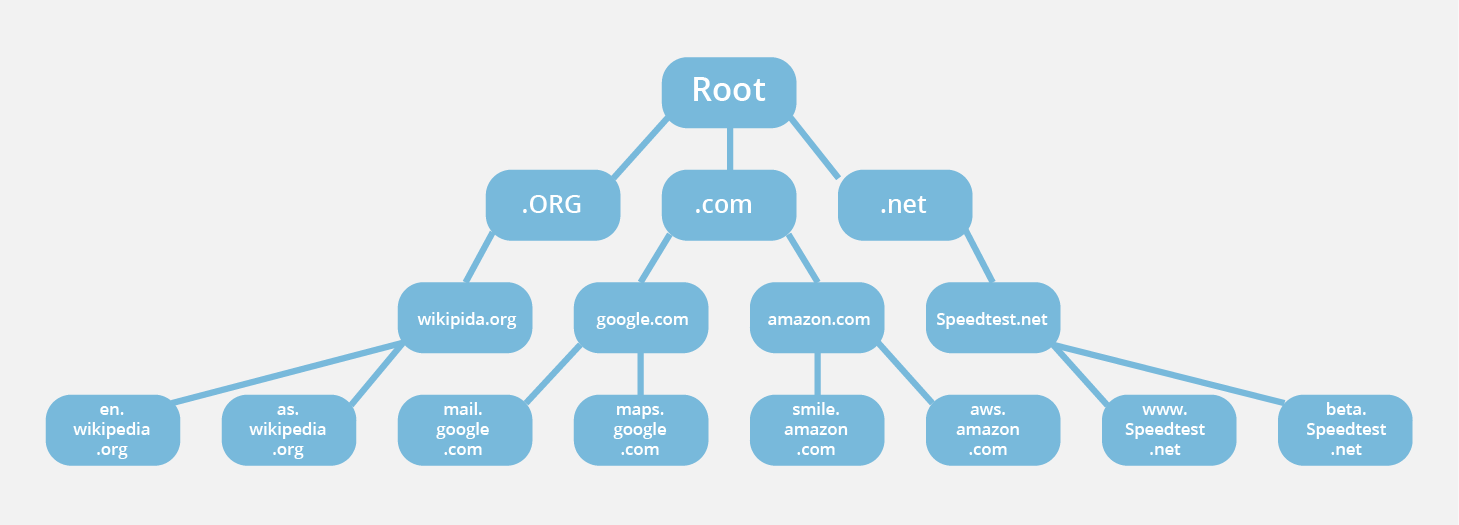
\includegraphics[width=0.45\textwidth]{figure/dns-root-server.png}
    \caption{\em The levels of authoritative DNS servers \cite{dns_root_server_cloudflare} \label{fig:levels_authoritative_DNS_servers}}
    \label{tab:Authoritative_DNS_server_levels}
\end{figure}

\begin{figure}[hbt!]  
    \centering
    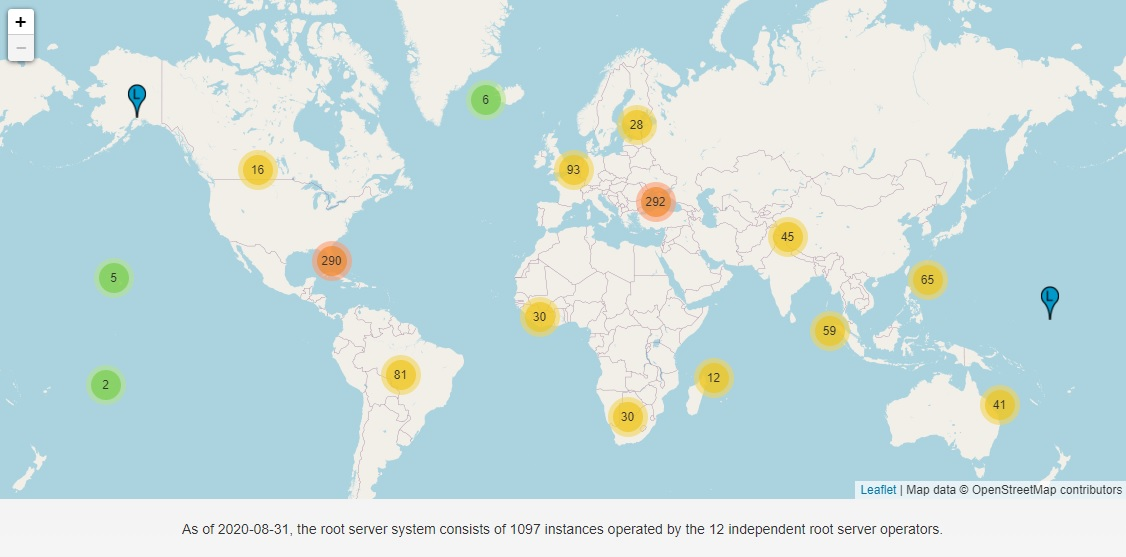
\includegraphics[width=0.45\textwidth]{figure/root-server-map-big.jpg}
    \caption{\em The root servers in the world \cite{root_servers_org} \label{fig:root_servers_in_the_world}}
\end{figure}

\begin{figure}[hbt!]  
    \centering
    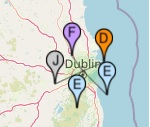
\includegraphics[width=0.20\textwidth]{figure/root-server-map-dublin.jpg}
    \caption{\em The root servers in Dublin \cite{root_servers_org} \label{fig:root_servers_dublin}}
\end{figure}

\begin{figure}[hbt!]  
    \centering
    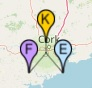
\includegraphics[width=0.20\textwidth]{figure/root-server-map-cork.jpg}
    \caption{\em The root servers in Cork \cite{root_servers_org} \label{fig:root_servers_cork}}
\end{figure}

In the map from Root-servers.org, there are 8 root servers in Ireland, 5 servers are in Dublin and 3 servers are in Cork. As for organizations, 3 servers belong to E-root(E zone, it is managed by NASA Ames Research Center), 2 servers belong to F-root(F zone, it is managed by Internet Systems Consortium). K-root(RIPE NCC), D-root(University of Maryland), J-root(Verisign) have 1 server respectively \cite{root_servers_org}.
\\

\begin{table}[hbt!]
    \centering
    \begin{tabular}{|c|c|c|}
        \hline
          Zone & Operator & Number in Ireland\\    
        \hline
        A & Verisign & 0 \\
        \hline
        B & USC-ISI & 0\\
        \hline
        C & Cogent Communications & 0 \\
        \hline
        D & University of Maryland & 1\\
        \hline
        E & NASA Ames Research Center & 3\\
        \hline
        F & Internet Systems Consortium & 2\\
        \hline
        G & Defense Information Systems Agency & 0\\
        \hline
        H & U.S. Army Research Lab & 0\\
        \hline
        I & Netnod & 0\\
        \hline
        J & Verisign & 1\\
        \hline
        K & RIPE NCC & 1\\
        \hline
        L & ICANN & 0\\
        \hline
        M & WIDE Project & 0\\
        \hline
    \end{tabular}
    \caption{The list of root server zones \cite{root_servers_org}}
    \label{tab:root_server_zone_list}
\end{table}

The problem is the information those organizations provided on Internet is limited. There is no statistic data of DNS queries in Ireland on their website.
\\

Next, the recursive structure of DNS servers has to be figured out. There are two kinds of DNS servers, the first kind of DNS server is recursive DNS server, it could be private or public, but those recursive DNS servers are not controlled by the organizations mentioned above. When users send queries to DNS servers, the queries will arrive recursive DNS servers first, if recursive DNS servers have matched IP addresses in their caches, then they can respond IP addresses to users directly. 
\\

The second DNS server is authoritative DNS server, they store the IP addresses of websites. Moreover, they are hierarchical, the highest one is root server. The levels of authoritative DNS servers are shown in Fig.~\ref{tab:Authoritative_DNS_server_levels}. If recursive DNS servers do not have matched IP addresses, they will ask authoritative DNS server for IP addresses and store it in their cache \cite{Authoritative_vs_Recursive_DNS_server}.
\\

Thus, the recursive structure of DNS server causes another problem, it is very hard to collect the records about all DNS queries, because there are numerous recursive DNS servers and they are managed by many organizations \cite{Authoritative_and_recursive_DNS}, hence, the operators of root servers do not have their data.
\\

However, it is not necessary to know the total number of DNS queries in Ireland, because the target in this research is to understand what the performance should a TTR server possess in Ireland. The number of DNS queries a root server may receive can help us to evaluate the required performance for a TTR server in Ireland.
\\

In this paper, the researcher designs some methods to estimate the traffic a DNS server would have in Ireland by using the traffic in root servers.
\\

Method 1 is using the data on Akamai.com to estimate the DNS traffic \cite{overall_DNS_traffic_trends}.
\\

In website Akamai.com, it collects the DNS traffic from 9 root server zones(B, C, D, E, F, I, K, L, M), but the DNS traffic is worldwide, it does not provide the data in national scale or city scale on the website.
\\

Even though there is no national scale data on Akamai.com, but the worldwide data can be used to estimate the Irish DNS traffic.
\\

In a report from Central Statistics Office of Ireland, it showed that there were 89\% of Irish households have the internet at home in 2018 \cite{Irish_households_with_internet}. From the growth of households with the internet, the percentage is probably 90\% in 2020. There were about 4.57 billion internet users in the world in July 2020 \cite{Global_digital_population_July_2020}. The population in Ireland was around 4.944 million in August 2020 \cite{Ireland_population}. Hence, the Irish Internet users may be about 4.113 million, it was approximately 0.09\% of internet users in the whole world.
\\

According to the data from Akamai.com \cite{overall_DNS_traffic_trends}, the overall DNS traffic in the world was about 7 Trillion transactions (Requests and responses) in June 2020. 
Then, 0.09\% of DNS traffic in the world could be Irish DNS traffic, which is around 6.3 billion DNS transactions for one month in Ireland. On average, it could be 210 DNS million transactions in a day in Ireland.
\\

\begin{figure}[hbt!]  
    \centering
    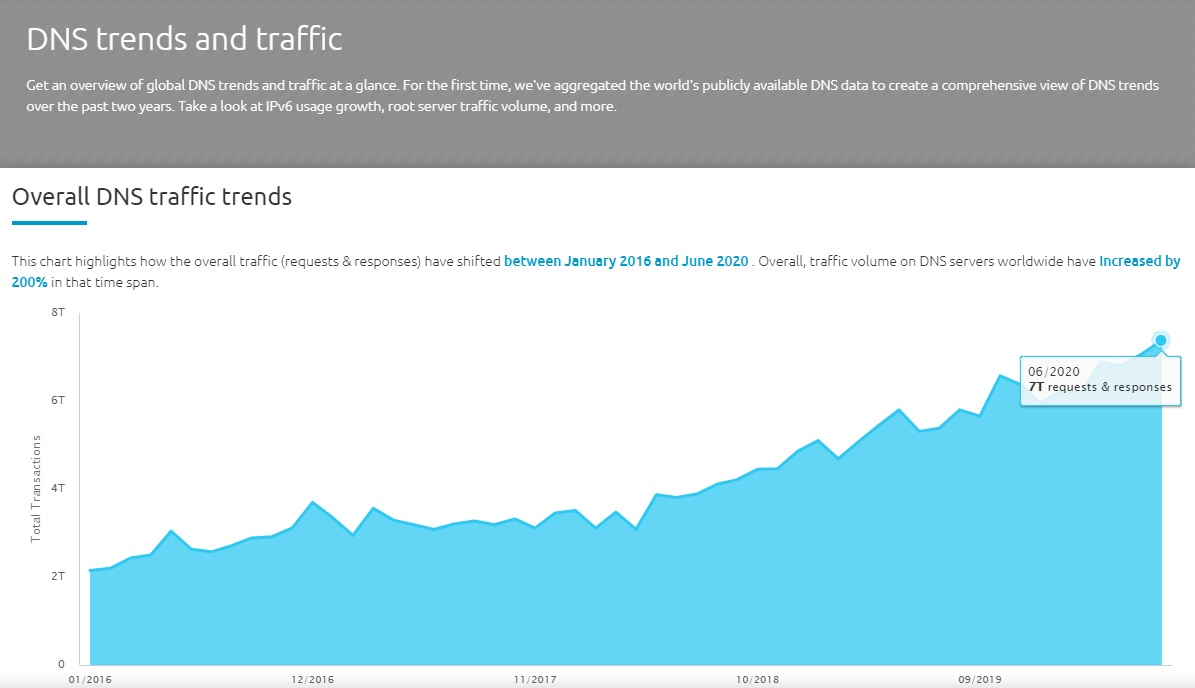
\includegraphics[width=0.45\textwidth]{figure/Overall DNS traffic trends.jpg}
    \caption{\em The trend of DNS traffic in the world \cite{overall_DNS_traffic_trends} \label{fig:trend_DNS_traffic}}
\end{figure}

\begin{table}[hbt!]
    \centering
    \begin{tabular}{|c|c|c|c|}
        \hline
         Month & IPv4 & IPv6 & Total\\
        \hline
         06/2020 & 6T & 1T & 7T \\
        \hline
        01/2020 & 5T & 969B & 6T\\
        \hline
        07/2019 & 4T & 919B & 5T \\
        \hline
        01/2019 & 4T & 848B & 5T \\
        \hline
        07/2018 & 3T & 564B & 4T \\
        \hline
        01/2018 & 3T & 426B & 4T \\
        \hline
        07/2017 & 3T & 371B & 3T \\
        \hline
        01/2017 & 3T & 363B & 3T \\
        \hline
        07/2016 & 2T & 248B & 3T \\
        \hline
        01/2016 & 2T & 171B & 2T \\
        \hline
    \end{tabular}
    \caption{Overall DNS traffic trends(Unit:Transactions) \cite{overall_DNS_traffic_trends}}
    \label{tab:DNS_traffic_trends}
\end{table}

However, internet traffic is changeable in different hours, it is necessary to understand when are the rush hours. For example, the internet rush hours are usually between 7 pm and 11 pm in UK \cite{Avoiding_the_internet_rush_hour}. In Sao Paulo, the internet rush hours are between 8 pm and 11 pm \cite{Brazil_internet_rush_hour}. In USA, it is 8 pm to 10 pm \cite{Measuring_broadband_america}. In Berlin, the rush hours are 8 pm to 11 pm \cite{Berlin_internet_traffic}. In Amsterdam, it is from 8 pm to 11 pm as well \cite{Amsterdam_internet_traffic}.
\\

\begin{figure}[hbt!]
    \centering
    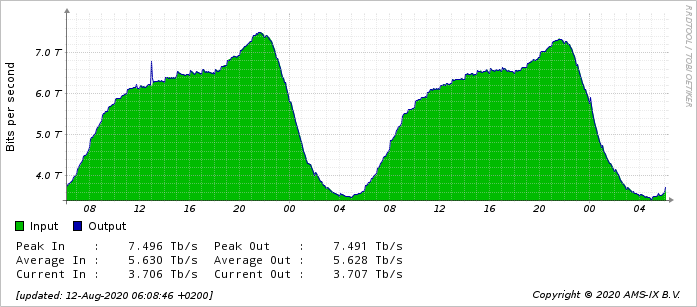
\includegraphics[width=0.45\textwidth]{figure/amsterdam-day.png}
    \caption{\em The internet traffic in a day (Amsterdam) \cite{Amsterdam_internet_traffic} \label{fig:internet_traffic_day_Amsterdam}}
\end{figure}

\begin{figure}[hbt!]    
    \centering
    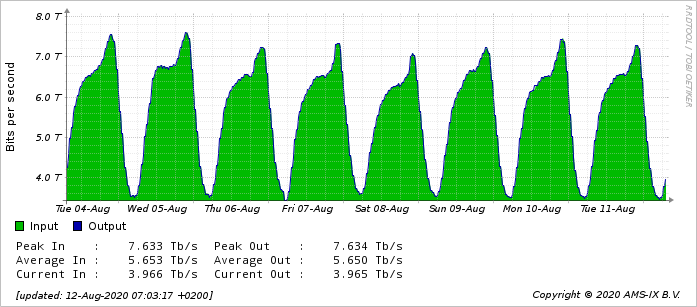
\includegraphics[width=0.45\textwidth]{figure/amsterdam-week.png}
    \caption{\em The internet traffic in a week (Amsterdam) \cite{Amsterdam_internet_traffic} \label{fig:internet_traffic_week_Amsterdam}}
\end{figure}

\begin{figure}[hbt!]  
    \centering
    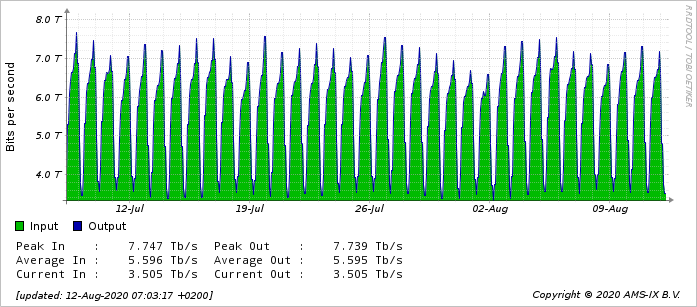
\includegraphics[width=0.45\textwidth]{figure/amsterdam-month.png}
    \caption{\em The internet traffic in a month (Amsterdam) \cite{Amsterdam_internet_traffic} \label{fig:internet_traffic_month_Amsterdam}}
\end{figure}

\begin{figure}[hbt!]
    \centering
    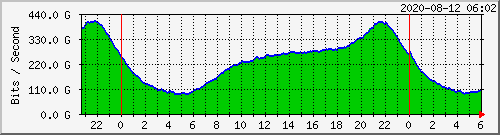
\includegraphics[width=0.45\textwidth]{figure/berlin-day.png}
    \caption{\em The internet traffic in a day (Berlin) \cite{Amsterdam_internet_traffic} \label{fig:internet_traffic_day_Berlin}}
\end{figure}

\begin{figure}[hbt!]
    \centering
    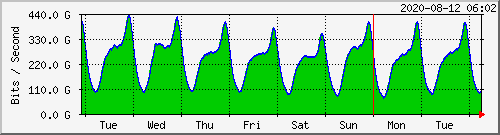
\includegraphics[width=0.45\textwidth]{figure/berlin-week.png}
    \caption{\em The internet traffic in a week (Berlin) \cite{Amsterdam_internet_traffic} \label{fig:internet_traffic_week_Berlin}}
\end{figure}

\begin{figure}[hbt!]
    \centering
    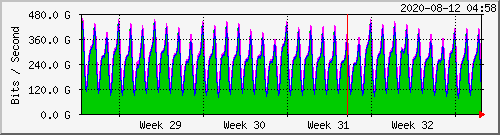
\includegraphics[width=0.45\textwidth]{figure/berlin-month.png}
    \caption{\em The internet traffic in a month (Berlin) \cite{Amsterdam_internet_traffic} \label{fig:internet_traffic_month_Berlin}}
\end{figure}

All the reports in different countries or cities revealed that internet rush hours are from 8 pm to 11 pm, the distributions are pretty similar. Therefore, Irish internet rush hours could be assumed as from 8 pm to 11 pm as well. 
\\

As for the comparison in different days in a week, from Monday to Sunday, the change is not obvious. About the days in a month, from the begin to the end of a month, there is no huge difference as well.
\\

Taking the data in Amsterdam to estimate the percentage of usage in each hour, the result is shown in TABLE ~\ref{tab:table_amsterdam}.
\\

\begin{table}[hbt!]
    \centering
    \begin{tabular}{|c|c|c|}
        \hline
         Hour(24) & Trillion bit/s & Percentage\\
        \hline
        0 & 5.8 & 4.3\% \\
        \hline
        1 & 4.8 & 3.56\% \\
        \hline
        2 & 4 & 2.96\% \\
        \hline
        3 & 3.7 & 2.74\% \\
        \hline
        4 & 3.6 & 2.67\% \\
        \hline
        5 & 3.5 & 2.59\% \\
        \hline
        6 & 3.6 & 2.67\%  \\
        \hline
        7 & 4 & 2.96\%  \\
        \hline
        8 & 4.8 & 3.56\%  \\
        \hline
        9 & 5.4 & 4\%  \\
        \hline
        10 & 5.8 & 4.3\%  \\
        \hline
        11 & 6 & 4.44\% \\
        \hline
        12 & 6.2 & 4.59\%  \\
        \hline
        13 & 6.4 & 4.74\%  \\
        \hline
        14 & 6.4 & 4.74\%  \\
        \hline
        15 & 6.6 & 4.89\%  \\
        \hline
        16 & 6.6 & 4.89\%  \\
        \hline
        17 & 6.6 & 4.89\%  \\
        \hline
        18 & 6.5 & 4.81\%  \\
        \hline
        19 & 6.7 & 4.96\%  \\
        \hline
        20 & 6.9 & 5.11\%  \\
        \hline
        21 & 7.2 & 5.33\%  \\
        \hline
        22 & 7.2 & 5.33\%  \\
        \hline
        23 & 6.7 & 4.96\% \\
        \hline
        Total & 135 & 100\%  \\
        \hline
    \end{tabular}
    \caption{Internet traffic and its percentage in each hour in a day in Amsterdam \cite{Amsterdam_internet_traffic}}
    \label{tab:table_amsterdam}
\end{table}

After that, using the percentage to multiply the estimated number of daily DNS transactions in Ireland, which is 210 million, then the result is sown in TABLE ~\ref{tab:table_dns_Ireland}. The 2 busiest hours are 9 PM and 10 PM, the number of DNS transactions could be  11.2 million in an hour.
\\

\begin{table}[hbt!]
    \centering
    \begin{tabular}{|c|c|c|}
        \hline
         Hour(24) & Percentage & Million transactions\\
        \hline
        0 & 4.3\% & 9.02 \\
        \hline
        1 & 3.56\% & 7.47 \\
        \hline
        2 & 2.96\% & 6.22 \\
        \hline
        3 & 2.74\% & 5.76 \\
        \hline
        4 & 2.67\% & 5.6 \\
        \hline
        5 & 2.59\% & 5.44 \\
        \hline
        6 & 2.67\% & 5.6  \\
        \hline
        7 & 2.96\% & 6.22  \\
        \hline
        8 & 3.56\% & 7.47  \\
        \hline
        9 & 4\% & 8.4  \\
        \hline
        10 & 4.3\% & 9.02  \\
        \hline
        11 & 4.44\% & 9.33 \\
        \hline
        12 & 4.59\% & 9.64  \\
        \hline
        13 & 4.74\% & 9.96 \\
        \hline
        14 & 4.74\% & 9.96 \\
        \hline
        15 & 4.89\% & 10.27 \\
        \hline
        16 & 4.89\% & 10.27 \\
        \hline
        17 & 4.89\% & 10.27 \\
        \hline
        18 & 4.81\% & 10.11 \\
        \hline
        19 & 4.96\% & 10.42 \\
        \hline
        20 & 5.11\% & 10.73 \\
        \hline
        21 & 5.33\% & 11.2 \\
        \hline
        22 & 5.33\% & 11.2 \\
        \hline
        23 & 4.96\% & 10.42 \\
        \hline
        Total & 100\% & 210  \\
        \hline
    \end{tabular}
    \caption{Using the daily distribution of Internet traffic of Amsterdam to estimate the DNS traffic in Ireland \cite{Amsterdam_internet_traffic}}
    \label{tab:table_dns_Ireland}
\end{table}

However, the data from Akamai.com does not include A, G, H and J root server zones. Thus, the number of transactions in rush hours should be higher than 11.2 million.
\\

The numbers of transactions in every root server zone are very different, therefore it is hard to estimate the numbers in A, G, H and J root server zones. If assume that the average number of A, G, H and J is close to the average number of B, C, D, E, F, I, K, L, M, then the estimated number of transactions in all root servers in rush hours could be 11.2/9X13=16.18 million.
\\

If convert it into a second, the number of DNS transactions could be 4,494 per second during the rush hour (16.18(million per hour)/60(minutes)/60(seconds)).
\\

Method 2 is using the data from ICANN to estimate DNS traffic. 
\\

ICANN (Internet Corporation for Assigned Names and Numbers) is the one of 12 organizations which are responsible for managing DNS root servers, the servers it manages are L-root servers. Unlike other 11 organizations, ICANN provides a website to display real-time DNS traffic, that is Stats.dns.icann.org \cite{stats_dns_icann_org}.
\\

The problem is ICANN does not have root servers in Ireland. Moreover, those data is only from ICANN, it does not include the data from other root server zones.
\\

Thus, here chose a city which has a similar population to Ireland to estimate the DNS traffic. Melbourne should be a ideal sample. The population in Melbourne is about 5 million in 2019 \cite{Melbourne_wiki}, which is close to the population in Ireland (4.9 million). Moreover, Melbourne is isolated, there is no big city near Melbourne,therefore the network connection may be similar to a country.
\\

\begin{figure}[hbt!]
    \centering
    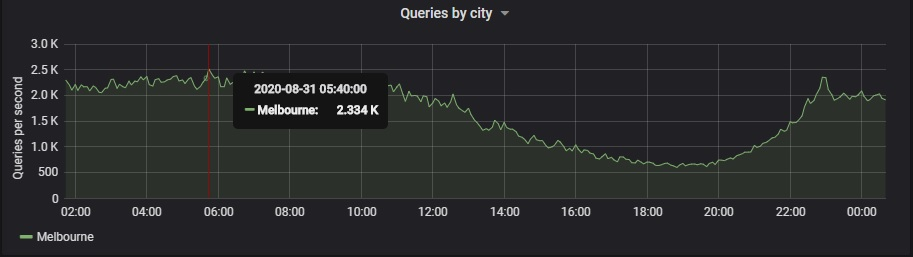
\includegraphics[width=0.45\textwidth]{figure/melbourne.jpg}
    \caption{\em The number of queries per second in a root server in Melbourne \cite{stats_dns_icann_org} }
    \label{tab:figure_melbourne}
\end{figure}

From the data in Fig.~\ref{tab:figure_melbourne}, the highest value in a day is 2,334 per second, which was occurred at 05:40 UTC(19:40 in Melbourne).
\\

\begin{figure}[hbt!]  
    \centering
    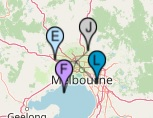
\includegraphics[width=0.20\textwidth]{figure/root-server-map-melbourne.jpg}
    \caption{\em The root servers in Melbourne \cite{root_servers_org} \label{fig:root_servers_Melbourne}}
\end{figure}

However, the data is only from a root server which is managed by ICANN, there are four root servers in Melbourne, the DNS traffic in other 3 root servers are not provided. Assume the average traffic in other 3 root servers is close to the root server managed by ICANN, the whole DNS traffic in Melbourne could be 9,336 per second(2,334X4). Next, adjust the traffic to accord the population of Ireland, the DNS traffic could be 9,149 per second during the rush hour(9,336/5X4.9).
\\

The comparison between method 1 and method 2 is shown in TABLE ~\ref{tab:estimation_comparison}.
\\


\begin{table}[hbt!]
    \centering
    \begin{tabular}{|p{2cm}|p{2.5cm}|p{2.5cm}|}
        \hline
          & Method 1 & Method 2\\    
        \hline
        Source & Akamai.com & ICANN \\
        \hline
         Queries per second in rush hours & 4,494 & 9,149\\
        \hline
         Drawback 1 & No Irish data & No Irish data \\
        \hline
         Drawback 2 & Only monthly data & The data is only from L-root\\
        \hline
    \end{tabular}
    \caption{The comparison between 2 methods for the estimation of the DNS traffic in Ireland}
    \label{tab:estimation_comparison}
\end{table}

\section{The concern of DDOS attacks}

DDOS is the important issue for building DNS server.
\\

There are 2 sorts of DNS queries, recursive and iterative. At the beginning, users send queries to recursive servers, when recursive DNS servers receive requests, if they do not have the matched IP addresses, then recursive DNS servers can help users to ask authoritative DNS servers for getting IP addresses, then return results to users, that is the recursive query. 
\\

As for the iterative query, when authoritative DNS servers receive the queries from recursive DNS servers, if they do not have the matched IP addresses, they will give recursive servers the IP addresses of other authoritative DNS servers for querying, then recursive servers will ask other authoritative DNS servers, this type of querying is the iterative query \cite{What_is_recursive_DNS}.
\\

However, the recursive queries may cause DDOS attacks. The content of packet could be faked, the IP address of a sender can be changed to be the IP address of the victim. In case thousands of computers send recursive queries to DNS servers, and all IPs of sources are changed to be the IP of a victim, then those DNS servers will send thousands of responses to that victim. After that, the traffic in the victim would be too high then cause some problems  \cite{Why_recursive_dns_not_recommended_video}. This type of DDOS attack is called DNS amplification attack \cite{DNS_amplification}.
\\

\begin{figure}[hbt!]  
    \centering
    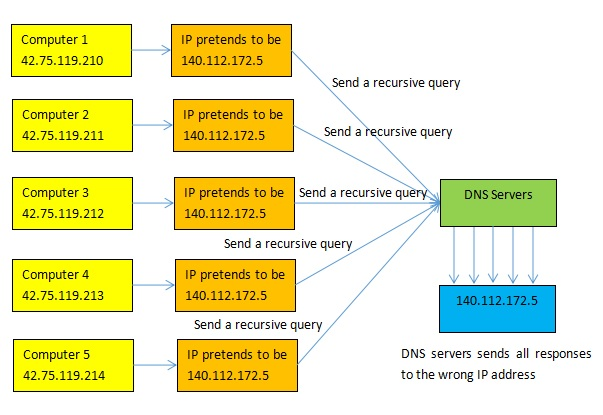
\includegraphics[width=0.45\textwidth]{figure/recursive-query-ddos.jpg}
    \caption{\em The DDOS attack in recursive DNS queries \cite{Why_recursive_dns_not_recommended_video} \label{fig:DDOS_attack}}
\end{figure}

Thus, restricting DNS queries may be the ideal method to prevent DNS amplification attacks, the implementation is to disable the recursion for everyone, only local queries are allowed to be processed \cite{Why_recursive_dns_not_recommended_web}.
\\

\begin{figure}[hbt!]  
    \centering
    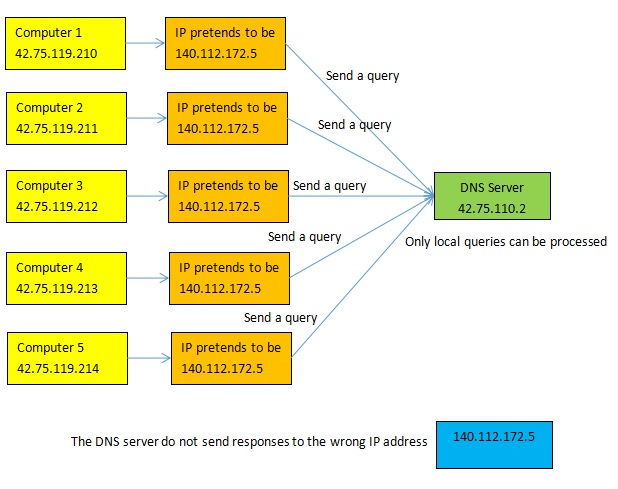
\includegraphics[width=0.45\textwidth]{figure/only_local_queries.jpg}
    \caption{\em Restricting DNS queries to prevent DNS amplification attacks \cite{Why_recursive_dns_not_recommended_video} \label{fig:restricting_DNS_queries}}
\end{figure}

\section{The required performance}

A DNS transaction contains many packets.
\\

\section{Required software}


Building a DNS server for TRR needs some software, including the software for implementing DNS server, tools and server \cite{DNS_resources}.
\\

First, implement DNS server, there are many choices, such as BIND, Unbound, DNSMASQ, PowerDNS, Microsoft DNS and Cisco Network Registrar \cite{DNS_software_wiki} \cite{Bind_dnsmasq_PowerDNS_Unbound}. In this research, Unbound, BIND and PowerDNS are recommended, because there are many discussion about those three software on Internet, moreover, they support DNS over HTTPS (DoH), then users may use TRR to browse websites in Firefox \cite{Building_DOH} \cite{DNS_over_HTTPS_servers}.
\\

Unbound is the free open-source software which focuses on building a recursive DNS server, it does not support the authoritative DNS server. The developer is NLnet Labs, the developer also designed another DNS software, which is NSD(Name Server Daemon), in contrast, NSD is only for building authoritative DNS servers \cite{NSD_wiki}. Unbound supports some security functions, such as Domain Name System Security Extensions(DNSSEC) and DNS over TLS(DoT). Moreover, the operating systems for running Unbound can be Linux, FreeBSD and Windows \cite{Unbound_wiki}.
\\

About BIND, its alias is Named. Unlike Unbound, it supports both recursive and authoritative DNS servers. It is developed by Internet Systems Consortium(ISC). ISC is also the organization which is responsible for managing F root server zone. The stable version is BIND 9. It can run on Windows, Mac-OS and Linux \cite{BIND_wiki}.
\\

PowerDNS, it supports both authoritative DNS server and recursive DNS server, moreover, it provides a Graphic UI for management and uses relational databases to store data. The developer is PowerDNS Community and operating systems are Linux and FreeBSD  \cite{PowerDNS_wiki}.
\\

Compare with Unbound, BIND and PowerDNS, those three software are all good choices \cite{Compare_the_different_DNS_servers}.
\\

For the consideration about the performance, there are some difference among BIND, Unbound and PowerDNS.
\\

According to a report which was written by Hamza Boulakhrif in University of Amsterdam, The times for processing queries in BIND, Unbound and PowerDNS were similar. The biggest difference was that when the time of processing exceeded 16 seconds, then PowerDNS did not response. If the time exceeded 17 seconds, BIND did not response, only Unbound can wait until the finish of processing then sent results to users \cite{DNS_resolver_performance_measurements}.
\\

The processing time in those 3 DNS software in this report is shown in Fig.~\ref{fig:DNS_resolver_performance_measurements}.
\\

\begin{figure}[hbt!]  
    \centering
    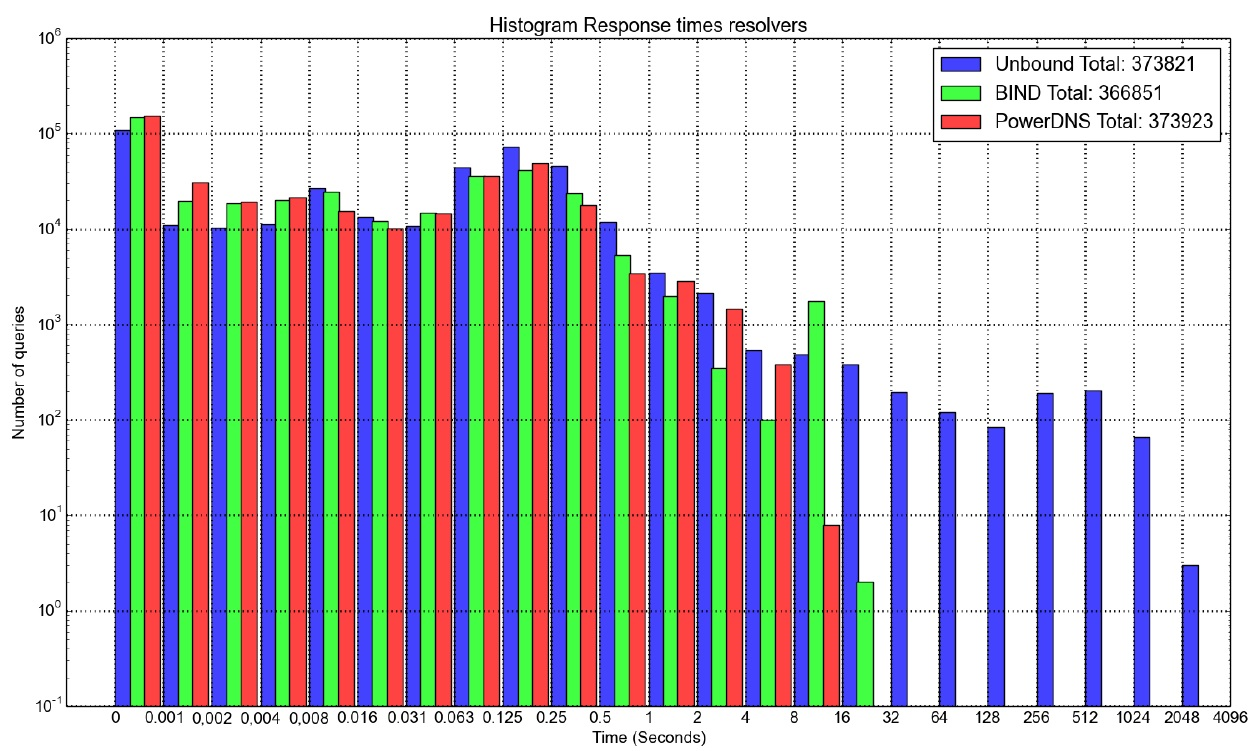
\includegraphics[width=0.45\textwidth]{figure/DNS-resolver-measurement.jpg}
    \caption{\em The processing time in BIND, Unbound and PowerDNS \cite{DNS_resolver_performance_measurements} \label{fig:DNS_resolver_performance_measurements}}
\end{figure}


In Fig.~\ref{fig:DNS_resolver_performance_measurements}, according to the assumption of Hamza Boulakhrif, if processing time is under 1 milliseconds, then it is processed by the cache, because the caches in DNS servers contain the matched IP addresses that users are looking for, thus DNS servers can response users in a very short time and do not need to ask authoritative DNS servers.
\\

\begin{figure}[hbt!]  
    \centering
    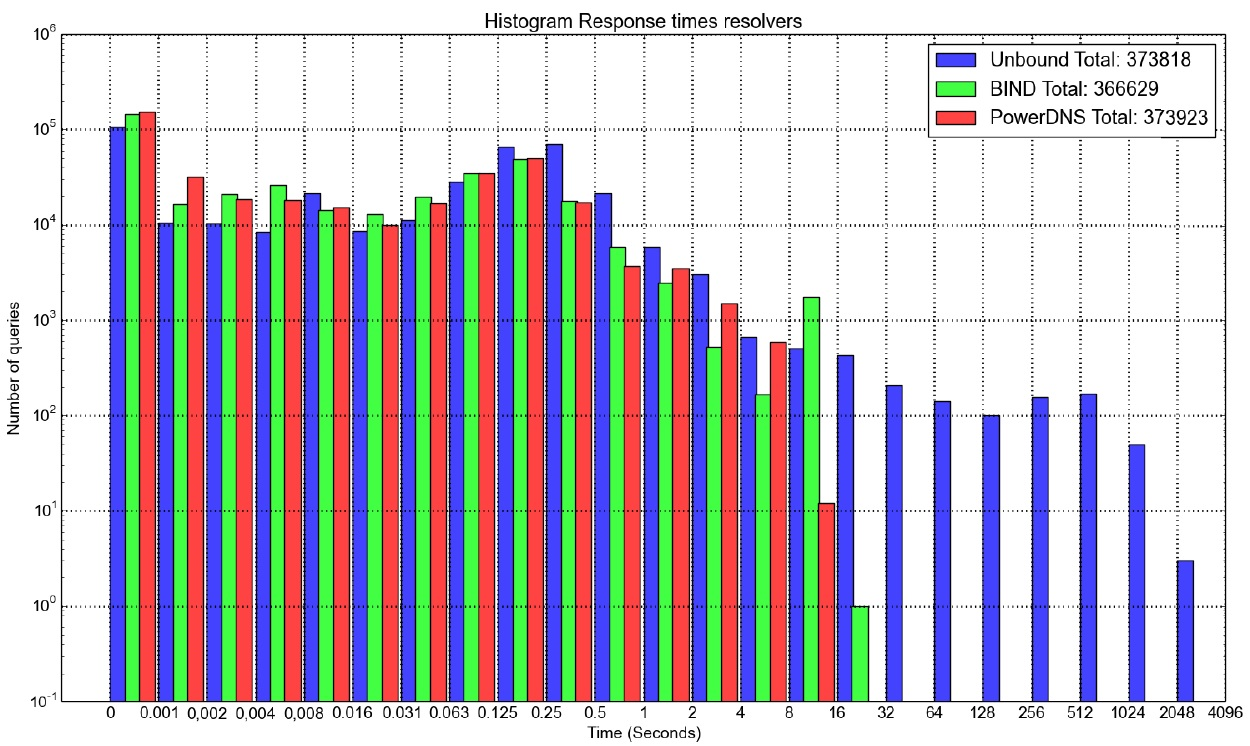
\includegraphics[width=0.45\textwidth]{figure/DNS-resolver-measurement-DNSSEC.jpg}
    \caption{\em The processing time in BIND, Unbound and PowerDNS with DNSSEC \cite{DNS_resolver_performance_measurements} \label{fig:DNS_resolver_performance_measurements_DNSSEC}}
\end{figure}


In the other experiment, BIND, Unbound and PowerDNS ran with DNSSEC, there was no obvious change if compare it with these DNS servers without DNSSEC. The result of using DNSSEC is shown in Fig.~\ref{fig:DNS_resolver_performance_measurements_DNSSEC}.
\\

\begin{figure}[hbt!]  
    \centering
    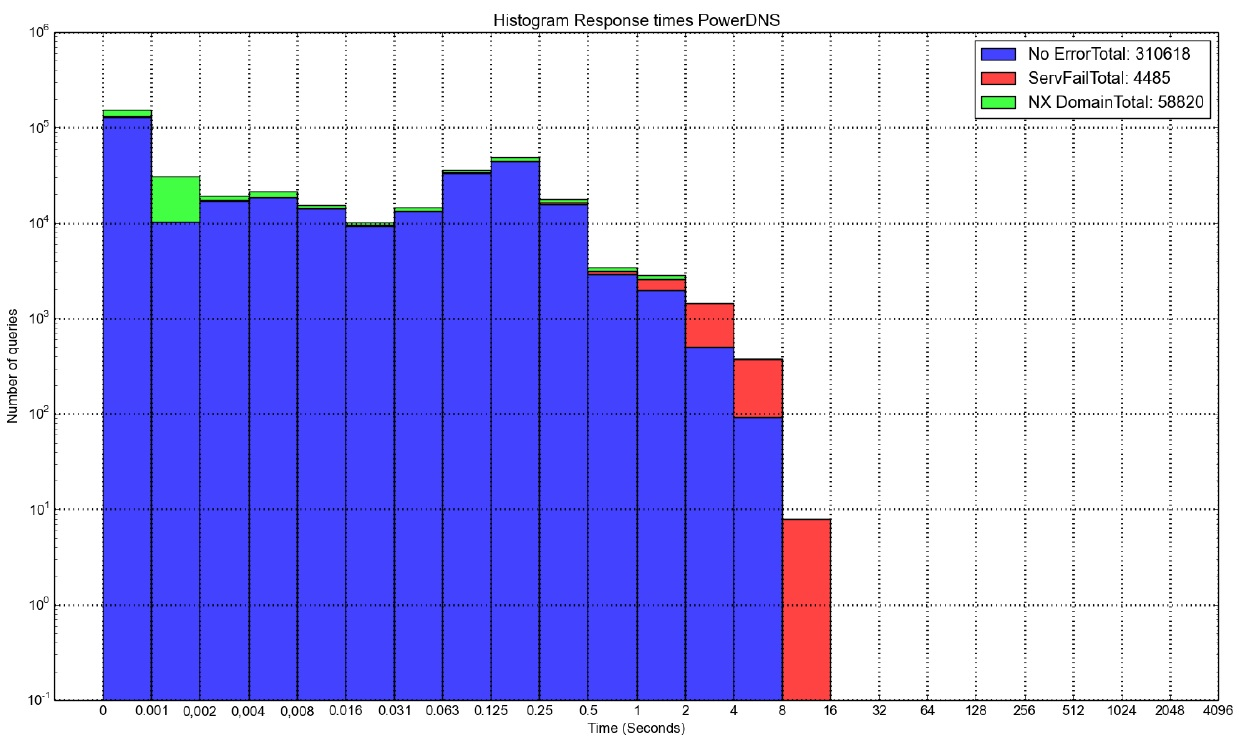
\includegraphics[width=0.45\textwidth]{figure/Measurement-PowerDNS.jpg}
    \caption{\em The processing time in PowerDNS \cite{DNS_resolver_performance_measurements} \label{fig:Measurements_PowerDNS}}
\end{figure}


\begin{figure}[hbt!]  
    \centering
    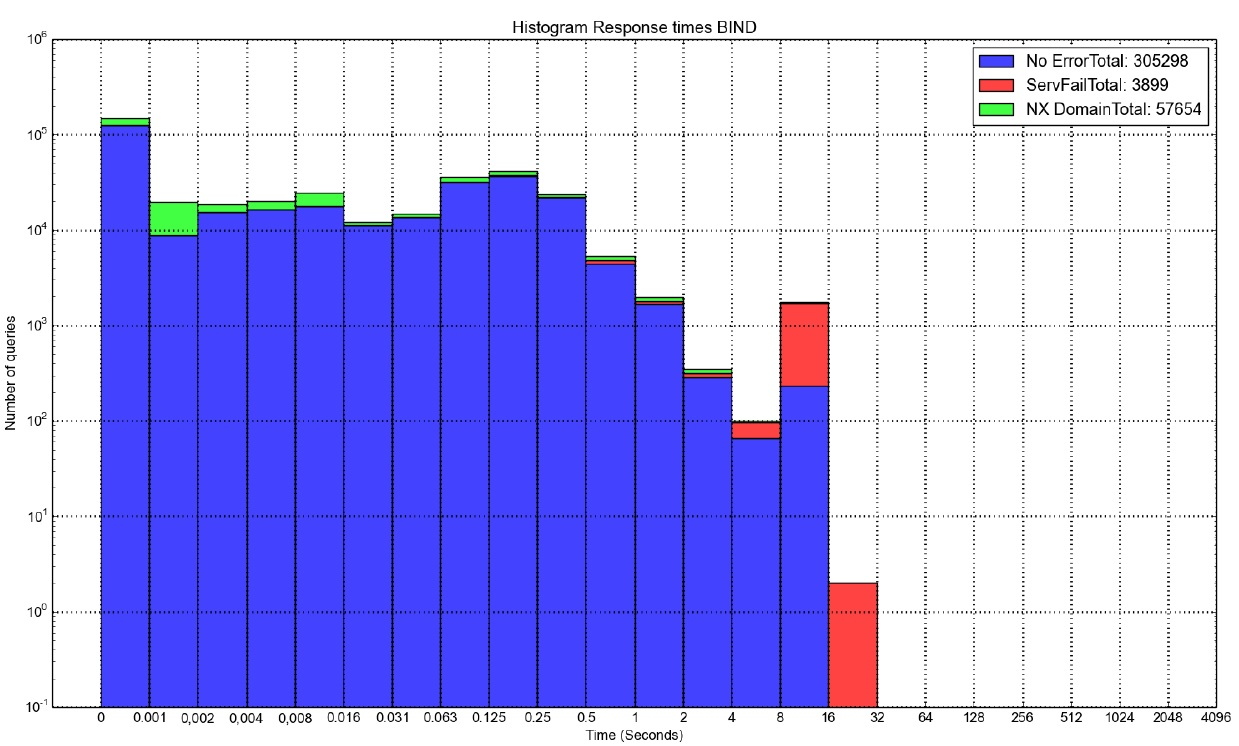
\includegraphics[width=0.45\textwidth]{figure/Measurement-BIND.jpg}
    \caption{\em The processing time in BIND \cite{DNS_resolver_performance_measurements} \label{fig:Measurement_BIND}}
\end{figure}


\begin{figure}[hbt!]  
    \centering
    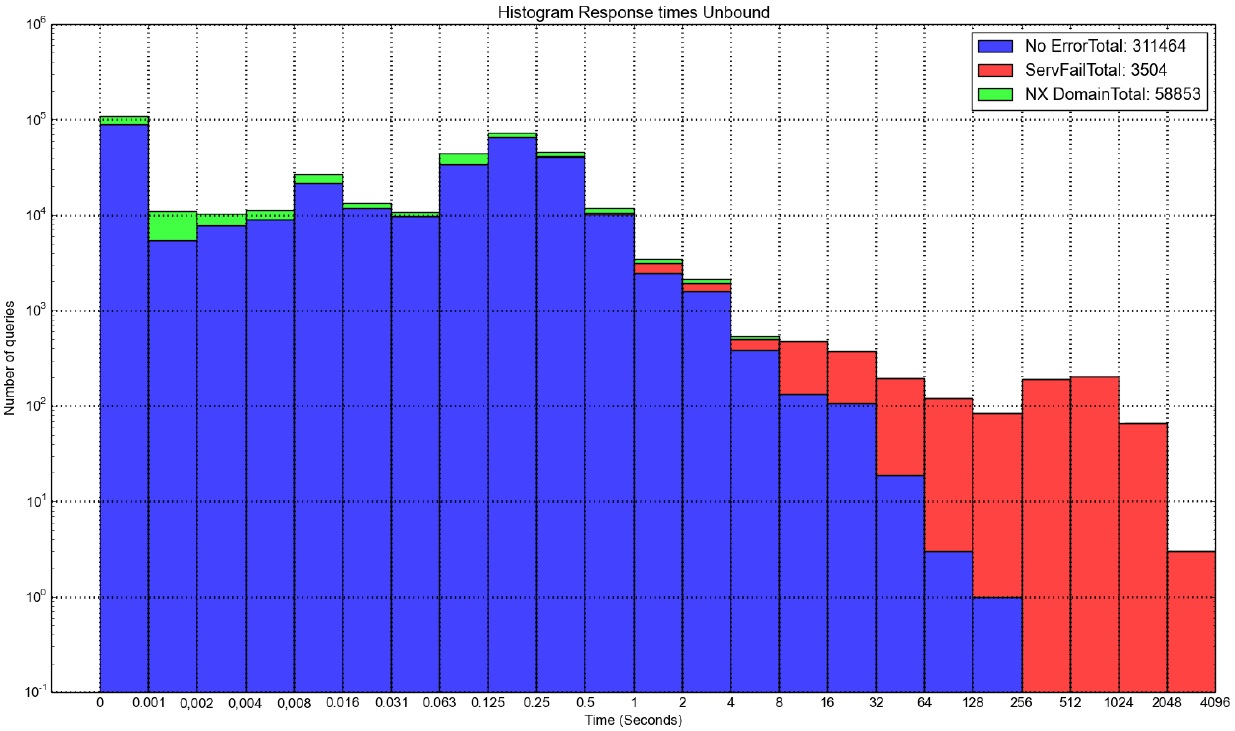
\includegraphics[width=0.45\textwidth]{figure/Measurement-Unbound.jpg}
    \caption{\em The processing time in Unbound \cite{DNS_resolver_performance_measurements} \label{fig:Measurement_Unbound}}
\end{figure}


Fig.~\ref{fig:Measurement_BIND}, Fig.~\ref{fig:Measurement_Unbound} and Fig.~\ref{fig:Measurements_PowerDNS} show the details of the time of processing queries in BIND, Unbound and PowerDNS. The working types in BIND and PowerDNS are similar, both of them have the time limit, thus in case the processing time reaches the time limit, then the query will be failed. In contrast, Unbound has a different working type, it allows the system to have a long time to wait for the answer after the process. Hamza Boulakhrif called those different working types as "Failed response over a late response" and "An answer is better than no answer". PowerDNS adopts "Failed response over a late response" and Unbound adopts "An answer is better than no answer", as for BIND, it is between PowerDNS and Unbound \cite{DNS_resolver_performance_measurements}.
\\

In conclusion, in choosing DNS resolver software, because BIND, Unbound, PowerDNS have similar performances, therefore the point of the decision is allowing a long time to wait for the answer or not. If yes, the operator should choose Unbound. Otherwise, he should choose BIND or PowerDNS.
\\

However, the report was written in 2015, which was 5 years ago, the situation may be different now.
\\

After the discussion about the performance, the next point is setting and usability.
\\

In order to understand the situation of the setting and usability among BIND, Unbound and PowerDNS, the researcher tried to install those 3 DNS software on a server and test them.
\\

In choosing a operation system for testing, there are many operation systems could be used to install DNS servers, such as Windows server, BSD, Linux Red Hat, Linux Ubuntu, Linux CentOS. Many developers prefer using Unix-like rather than Windows server base on the concern about stability and cost, therefore the researcher excluded Windows server.
\\

On the other hand, even though BSB is a good choice for building servers, but the information of BSD is less than Linux, which means Linux is more popular, thus the researcher decided to use Linux.
\\

However, there are many members in the Linux family, including Fedora,Red Hat Linux, CentOS, Ubuntu, Debian \cite{Linux_distributions}. CentOS is chosen here, because it is free, and the structure is the offshoot of Red Hat enterprise, hence it is very stable. 
\\

After that, started to install the operating system. Due to the effect of COVID-19, students were not allowed to go inside the laboratory, hence this study has to be finished at home, therefore the equipment was limited, only 4 personal devices were available to the researcher, which were a personal desktop computer, 2 android phones and a IPad. The operating system on the personal desktop computer is Windows 10. Thus, there was no spare computer to install Linux, the researcher had to use a virtual machine to install Linux on the personal computer. The software for running virtual machine was VMware Workstation Player.
\\

After installing the operation system, then installed BIND, Unbound and PowerDNS, and set the configuration files of those DNS servers, to make sure those DNS servers were in the same network zone with other testing devices.
\\

Next, used Internet Information Services(IIS) to create a simple website on the personal computer, and gave fixed local IP addresses to all devices and the virtual machine, then both the DNS server and website had the IP addresses. In the DNS server(BIND, Unbound and PowerDNS), set a domain name to the simple website to match its IP address. The simple website was the testing website.
\\

Finally, used the testing devices(Android phone and IPad) to type the domain name of the testing website on browsers(Google Chrome and Safari). If the testing website could be displayed on testing devices, then the DNS server functioned well. \\

Above steps were the testing method for the study. The testing environment is shown in TABLE ~\ref{tab:Testing_environment}.

\begin{table}[hbt!]
    \centering
    \begin{tabular}{|c|c|}
        \hline
         Platform & VMware Workstation 15.5.6 Player \\    
        \hline
         Operating system & CentOS 8.2.2004 \\
        \hline
         Internet connection & Bridge mode \\
        \hline
         Testing devices & Desktop, IPad, Android phone\\
        \hline
    \end{tabular}
    \caption{The testing environment}
    \label{tab:Testing_environment}
\end{table}

Next, the following discussion is about configuration. The configuration of BIND is using C language to be the format of the configuration file. Therefore, in case the maintenance personnel does not have programming background, then it needs time to understand the syntax of C language.
\\

About Unbound, the format of configuration file is very simple, it does not belong to any kind of computer languages. The setting is just listed line by line.
\\

PowerDNS adopts relational database, thus the configuration of PowerDNS has 2 parts, the first part is the normal configuration file, it decides the setting for the database. The second part is in the database, the contain is including domains and records.
\\

The installation of PowerDNS is more complex than Unbound and BIND, because it uses the rational database. However, it is a double-edged sword, it is not friendly for normal users during the installation, but after installation, PowerDNS provides the website to display the information of DNS server, and the website is also the interface for the setting, hence the maintenance is easier than BIND and Unbound.
\\

The comparison among BIND, Unbound, PowerDNS is shown in Table ~\ref{tab:BIND_unbound_powerDNS}.

\begin{table}[hbt!]
    \centering
    \begin{tabular}{|c|c|c|c|}
        \hline
         & BIND & Unbound & PowerDNS \\    
        \hline
         Version &  &  & \\
        \hline
         Query time limit & Short & Long & Short \\
        \hline
         Performance & Similar & Similar & Similar \\
        \hline
         Configuration & C language & Line by line  & RDBMS \\
        \hline
         Log style & Log file & Log file & MySQL \\
        \hline
         Installation difficulty & Easy & Easy & Difficult \\
        \hline
         Maintenance difficulty & Normal & Normal & Easy \\
        \hline
    \end{tabular}
    \caption{The comparison among BIND, Unbound, PowerDNS}
    \label{tab:BIND_unbound_powerDNS}
\end{table}


The DNS server need tools to recieve DoH queries and test. DoH-proxy is designed for this purpose, the developer is Facebook. It can be installed on Linux but it requires Python 3.5 \cite{doh_proxy}.
\\

After that, NGINX can provide the web service. NGINX is a HTTP server with high performance, it can also provide different kinds of services. The operator can set the method for listening queries in a port and the request from users \cite{NGINX_wiki}.
\\

About Operating System, Linux is recommended, because the much resource for building DNS servers is based on Linux \cite{configure_BIND}.
\\

The required software is shown in TABLE ~\ref{tab:required_software}.
\\

\begin{table}[hbt!]
    \centering
    \begin{tabular}{|c|c|c|}
        \hline
         Category & Software & Note\\    
        \hline
         DNS & BIND 9 & \\
        \hline
         DNS & Unbound & Free and open-source software\\
        \hline
         DNS & PowerDNS & \\
        \hline
         Tool & DoH-proxy &  \\
        \hline
        Server & NGINX & Free and open-source software\\
        \hline
    \end{tabular}
    \caption{The required software for building a DNS server for TRR}
    \label{tab:required_software}
\end{table}


\section{The concern of other issues}


COVID-19
\\

\section{Conclusion}


\bibliographystyle{ieeetr}
\bibliography{trr.bib}


\end{document}
